\documentclass[11pt,letterpaper]{article}

\usepackage[utf8]{inputenc}
\usepackage[spanish,es-nodecimaldot]{babel}
\usepackage{graphicx}
\usepackage{amsmath}
\usepackage{amssymb}

\usepackage[top=1in, bottom=1in, left=1in, right=1in]{geometry}

\begin{document}

\begin{titlepage}
    \centering

    {\scshape\LARGE Universidad Nacional Autónoma de México \par}

    \vspace{1cm}
    {\scshape\Large Facultad de Ciencias\par}
    \vspace{1.5cm}

    \begin{center}
        
\includegraphics[scale=.1]{../../assets/img/logo.png}
    \end{center}

    \vspace{.8 cm}

    {\LARGE Práctica 01: \par}
    {\huge\bfseries Compilador \par}

    \vspace{0.5cm}
    {\large\itshape Pablo A. Trinidad Paz\par}

    \vfill

    Trabajo presentado como parte del curso de \textbf{Introducción a Ciencias de la Computación}
    impartido por la profesora \textbf{Verónica Esther Arriola Ríos}. \par
    \vspace{0.1cm}
    {\large 24 de agosto de 2018\par}
\end{titlepage}

{\Large \bfseries Los programas de la JDK \par}

\begin{enumerate}
    \item [Actividad 1.2)] {\bfseries Escribe exactamente que archivos fueron creados y donde:\par}

        Dentro de \verb|Reloj/src/icc/practica1| los siguientes archivos fueron creados:
        \begin{enumerate}
            \item [1.] \verb|ClaseReloj.class|
            \item [2.] \verb|PanelDeReloj.class|
            \item [3.] \verb|Reloj.class|
            \item [4.] \verb|TiempoSistema.class|
            \item [5.] \verb|UsoReloj.class|
            \item [6.] \verb|VistaReloj.class|
            \item [7.] \verb|VistaRelojAnalogico.class|
            \item [8.] \verb|VistaRelojAnalogico$1.class|
        \end{enumerate}

    \item [Actividad 1.3)] {\bfseries Ejecuta \verb|UsoReloj|\par}
            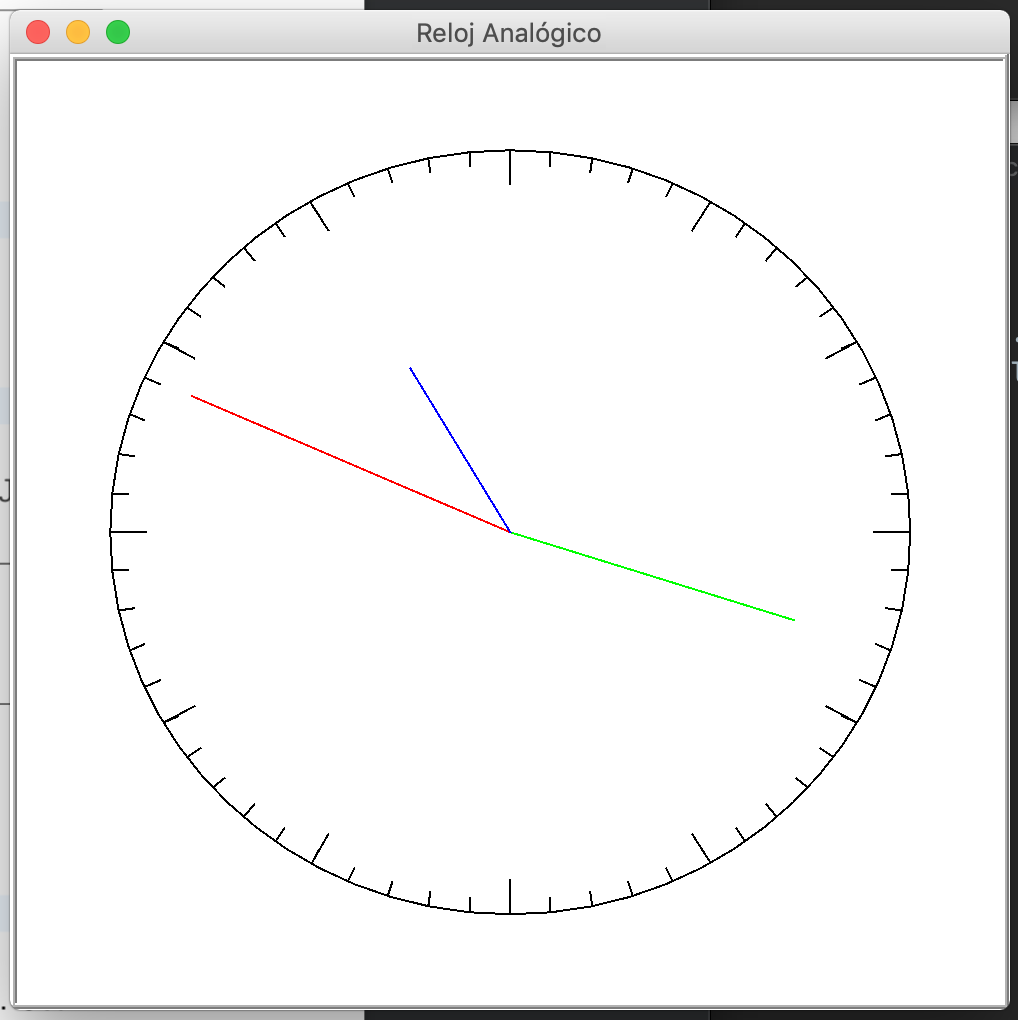
\includegraphics[scale=.3]{assets/img/1-3.png}

\end{enumerate}


\end{document}
